\section{Architecture Overview}
\label{socksdirect:sec:architecture}

To simplify deployment and development \cite {andromeda}, and to eliminate kernel crossing overhead, this chapter implements \sys{} in user space rather than in the kernel.
To use \sys{}, the application loads the user-space library \libipc {} by setting the \texttt {LD\_PRELOAD} environment variable. \libipc {} intercepts all Linux APIs related to file descriptor operations in the standard C library (glibc), implementing socket functionality in user space.
From a security perspective, because \libipc {} resides in the application address space, its behavior is untrusted. For example, a malicious program might directly write arbitrary messages into the RDMA QP, bypassing the security checks in the \libipc{} library.
In addition, as shown in Table \ref{socksdirect:tab:socket-api}, although most socket operations can be implemented between the caller's local or both ends of the connection, many socket operations require centralized coordination. For example, the TCP port number is a global resource that needs to be centrally allocated \cite {lin2016scalable,nsdi19freeflow}. Therefore, a trusted component outside of \libipc {} is needed to enforce access control and manage global resources.

\begin{table*}[htbp]
	\centering
	\small
	\begin{tabular}{ll|ll}
		\toprule
		\multicolumn{2}{c|}{Initialization} &
		\multicolumn{2}{c}{Connection Management} \\
		\midrule
		API & Category &
		API & Category \\
		\midrule
		\textbf{socket} & Local &
		\textbf{connect} & NoPart \\

		bind & NoPart &
		\textbf{accept(4)} & P2P \\

		listen & NoPart &
		\textbf{\textit{fcntl, ioctl}} & Local \\

		socketpair & Local &
		\textbf{(get,set)sockopt} & Local \\

		getsockname  & Local &
		\textbf{\textit{close}, shutdown} & P2P \\

		\textbf{\textit{malloc}} & Local &
		getpeername & Local \\

		\textbf{\textit{realloc}} & Local &
		\textit{dup(2)} & P2P  \\

		\textit{epoll\_create} & Local &
		\textbf{\textit{epoll\_ctl}} & Local \\
		\bottomrule
		\toprule
		\multicolumn{2}{c|}{Data Transfer} &
		\multicolumn{2}{c}{Process Management} \\
		\midrule
		API & Category &
		API & Category \\
		\midrule
		\textbf{recv(from,(m)msg)} & P2P &
		\textit{pthread\_create} & NoPart \\

		\textbf{\textit{write(v)}} & P2P &
		\textit{clone} & NoPart \\

		\textbf{\textit{read(v)}} & P2P &
		\textit{execve} & NoPart \\

		\textbf{\textit{memcpy}} & Local &
		\textit{exit} & P2P \\

		\textit{(p)select} & P2P &
		\textit{sleep} & P2P \\

		\textit{(p)poll} & P2P &
		\textit{daemon} & P2P \\

		\textbf{\textit{epoll\_(p)wait}} & P2P &
		\textit{sigaction} & Local \\
		\bottomrule
	\end{tabular}
	\caption{Main Linux APIs related to sockets and intercepted by \libipc{}. Categories include Local, Peer-to-Peer (P2P), and Non-partitionable (NoPart). \textit{Italic} APIs indicate other uses of the operating system besides sockets. \textbf{Bold} APIs are called more frequently than other APIs, and therefore are more worth optimizing.}
	\label{socksdirect:tab:socket-api}
\end{table*}

For this purpose, a \emph{monitor} daemon (hereinafter referred to as \textit{monitor}) is designed on each host to coordinate control plane operations, such as connection creation. To ensure isolation, we treat all applications and monitors as a distributed system that does not share data structures, using message communication as the only communication mechanism. On each host, all applications loaded with \libipc{} must establish a shared memory (shared memory) queue with the host's monitor, thus forming a control plane. On the data plane, applications build end-to-end (peer-to-peer) queues for direct communication, thereby alleviating the burden of the monitor daemon. The monitor is a single-threaded user-mode program that polls messages from the end-to-end queues of all applications. Figure \ref{socksdirect:fig:architecture} shows the architecture of \sys{}.

\begin{figure}[htbp]
	\centering
	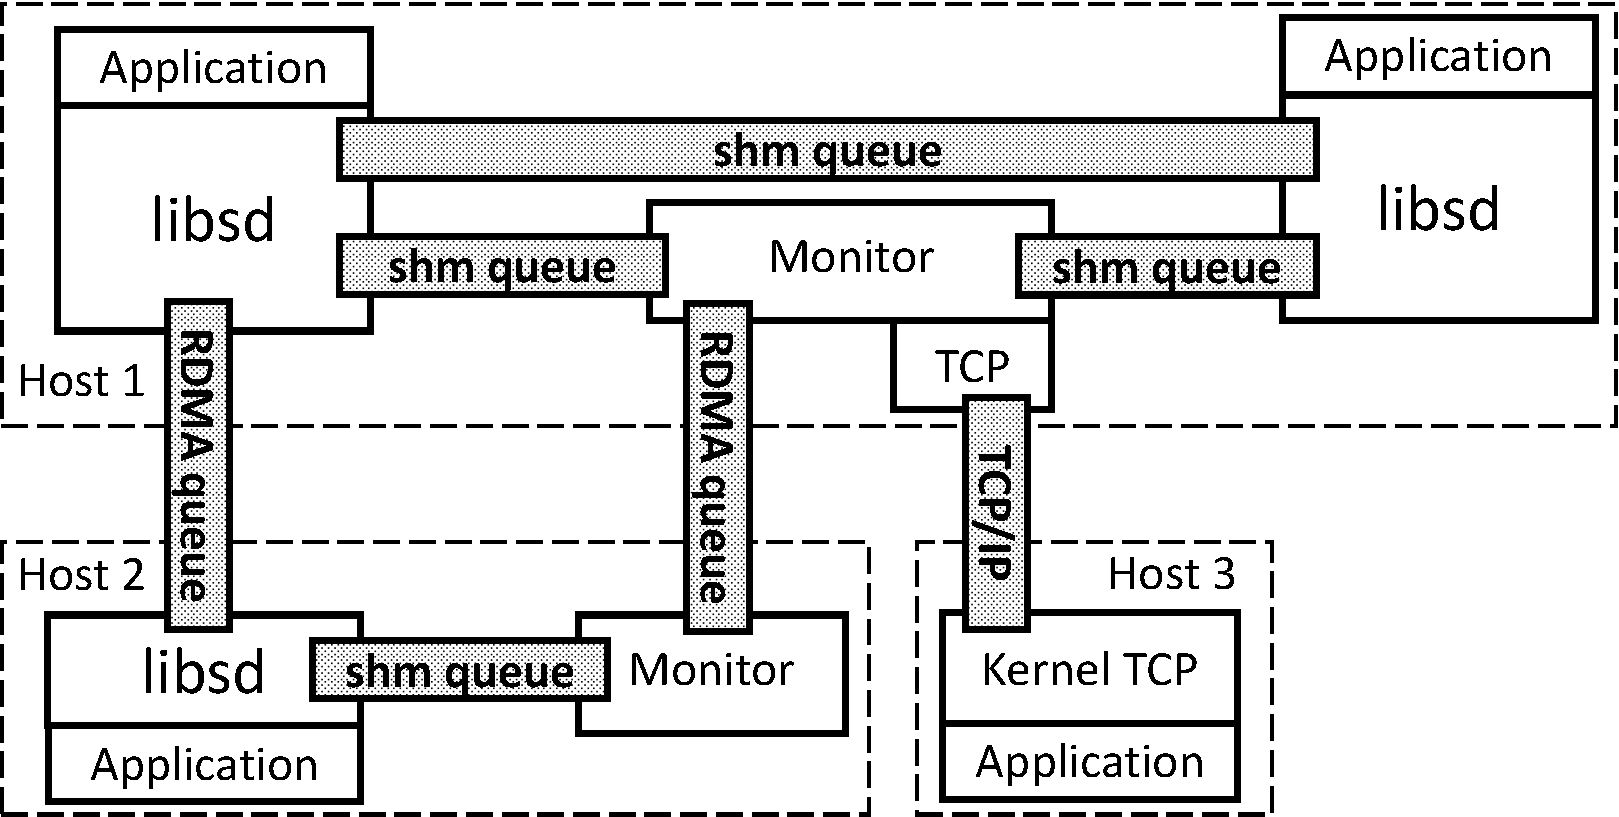
\includegraphics[width=0.8\textwidth]{images/architecture_new}
	\caption{The architecture of \sys{}. Hosts 1 and 2 have RDMA capabilities, while Host 3 does not.}
	\label{socksdirect:fig:architecture}
\end{figure}

To achieve low latency and high throughput, \sys{} uses shared memory for intra-host communication and RDMA for inter-host communication. Each socket connection is mapped to a shared memory queue or RDMA QP. The shared memory or RDMA QP is marked by a unique token, so other non-privileged processes cannot access it. Socket send operations are converted into shared memory or RDMA write operations on the socket buffer at the remote endpoint.

For \emph{intra-host} communication, the initiator first sends a request to the local monitor, and then the monitor establishes a shared memory queue between the two applications (possibly in different containers). After this, the two applications can communicate directly.

For \emph{inter-host} communication, the monitors of both hosts are involved. When an application connects to a remote host, its local monitor establishes a regular TCP connection and detects whether the remote host supports \sys{} and RDMA. If both are supported, an RDMA queue is established between the two monitors, so that future socket connections between the two hosts can be created faster. The monitor at the remote end schedules the connection with the target and helps the two applications establish an RDMA queue, as between Hosts 1 and 2 in Figure \ref{socksdirect:fig:architecture}. If the remote host does not support \sys{}, it will continue to use the TCP connection, as between Hosts 1 and 3 in Figure \ref{socksdirect:fig:architecture}. The detailed connection management protocol is introduced in Section \ref{socksdirect:subsec:connection-management}.

To ensure thread safety and avoid locks, as well as support fork and container hot migration, this chapter optimizes for the common case where only one pair of send and receive threads are active, while ensuring correctness in all cases (Section \ref{socksdirect:subsec:fork}). To eliminate buffer management overhead, a ring buffer is designed, where each inter-host message only requires one RDMA write operation, and each intra-host message requires one cache migration (Section \ref{socksdirect:subsec:lockless-queue}). This chapter further designs a zero-copy mechanism that can eliminate data copying of larger messages at the sending and receiving ends (Section \ref{socksdirect:subsec:zerocopy}). Finally, Section \ref{socksdirect:subsec:process-mux} provides an event notification mechanism.

As shown in Figure \ref{socksdirect:fig:libsd-architecture}, the \libipc{} runtime library consists of four layers: API encapsulation, Virtual File System (VFS), queue, and transmission. The API encapsulation layer uses a \emph{file descriptor remapping table} to distinguish between socket file descriptors and kernel file descriptors (such as files and devices), implements socket functions in user space, and forwards other system calls to the kernel through the standard C library (glibc). The Virtual File System layer implements functions such as connection creation and closure, event polling and notification, multi-process shared sockets, fork, container migration, etc., and is the most complex layer. Next to the Virtual File System is the signal layer, which is responsible for receiving events from the operating system and communicating with the monitor and the other end. The next layer is the lock-free queue based on the ring buffer. The bottom layer is the transmission layer, implemented with Shared Memory (SHM) or RDMA.

\begin{figure}[htbp]
	\centering
	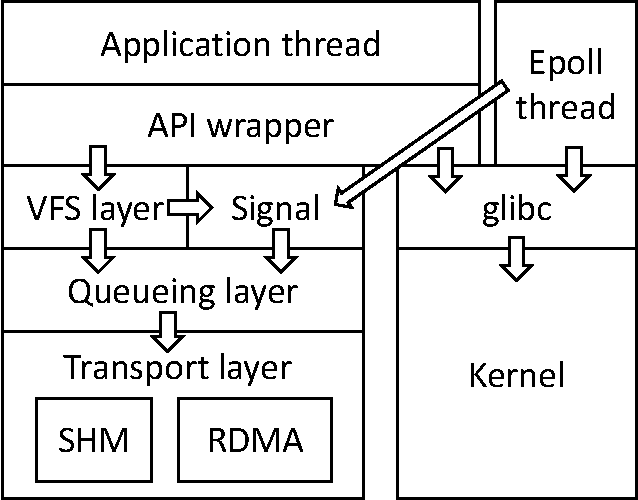
\includegraphics[width=0.5\textwidth]{images/libsd_architecture}
	\caption{The architecture of \libipc{} runtime library.}
	\label{socksdirect:fig:libsd-architecture}
\end{figure}

%In order to remove synchronization overhead for multi-threaded applications, we treat each thread as a separate process.
%%Although threads in a process share memory, we use thread-specific storage for most states in \libipc{}.
%For two communicating applications, we create peer-to-peer queues between each pair of sender and receiver threads to avoid synchronization cost of contending on the same queue.
%In Sec.~\ref{socksdirect:subsec:fork}, we present the peer-to-peer queue design that preserves FIFO ordering semantics and avoids starvation, especially when a process forks or creates a new thread.
%To maintain performance with many concurrent connections, rather than creating separate queues for each connection, we multiplex data from all connections through one queue.
%In Sec.~\ref{socksdirect:subsec:multiplex-conn}, we present the design of multiplexed queue that avoids head-of-line blocking and supports fetching data from any multiplexed connections.

%Inspired by Unikernels~\cite{madhavapeddy2013unikernels}, we move networking and IPC functions from the kernel to user space. Similar to existing works~\cite{peter2016arrakis,jeong2014mtcp,libvma}, we leverage multiple queues in modern network cards to enable user-space direct access to network. %The kernel is still responsible for process creation, scheduling, virtual memory and device management, but no longer on the critical path of performance.
%To maintain compatibility with existing Linux applications, we design a user-mode library \libipc as a drop-in replacement of the system call wrappers in the GNU C library (glibc). \libipc{} implements network socket functions in user mode, and adds a wrapper to other system calls to track process creation and memory allocation. \libipc{} is not considered a secure domain, as it shares memory space with the application. When \libipc{} is loaded, it creates a Linux native \textit{bootstrap socket} to the \textit{monitor} daemon, then creates a shared memory queue to the monitor.

%Even though multiple threads in the same process share memory space, we still treat each thread as a separated process and use thread-specific storage to store states in \libipc. In the following text, unless explicitly mentioned, we use a ``process'' to refer to a regular process or a thread.

\section{System Design}
\label{socksdirect:sec:design}


\subsection{Token-based Socket Sharing}
\label{socksdirect:subsec:fork}


Most socket systems maintain a lock for each file descriptor to enable socket sharing among threads and processes.
Previous work \cite {boyd2010analysis,clements2015scalable} has shown that many socket operations are not commutative and synchronization cannot always be avoided.
This chapter takes advantage of the fact that shared memory message passing is much cheaper than locks \cite {roghanchi2017ffwd}, and uses message passing as the only synchronization mechanism.


Logically, a socket consists of two FIFO \emph {queues} in opposite transmission directions, each with multiple concurrent senders and receivers.
The system design goal is to maximize general case performance while maintaining FIFO semantics.
This paper observes the following two characteristics of applications: first, high-performance applications rarely fork and create threads due to high costs.
Second, it is not common for several processes to concurrently send or receive from a shared socket, as the byte stream semantics of sockets make it difficult to avoid receiving partial messages.
Applications that need to send or receive simultaneously usually use a message broker \cite {hintjens2013zeromq,rabbitmq2017rabbitmq,kreps2011kafka} instead of directly sharing sockets.
The common case of inter-process socket sharing is that applications implicitly migrate sockets from one process to another, such as offloading transactions from the main process to a worker process.




\iffalse
Based on the observations, we propose the following requirements:

\begin{enumerate}[noitemsep,nolistsep]
 \item \textbf{Synchronization-free.} With multiple senders and receivers, if only one pair of sender and receiver is active, no synchronization should occur.
 \item \textbf{Multi-sender scalability.} Multiple processes may send data concurrently through a shared socket. With multiple active senders and a single receiver, if the receiver is not a bottleneck, the throughput should scale.
 \item \textbf{Self-stabilization.} Certain operations (\textit{e.g.} \texttt{fork}) may slow down the system temporarily, but after that the performance should converge back to normal.
\end{enumerate}

For compatibility with Linux semantics, we also need to ensure message ordering and liveness:
\begin{enumerate}[noitemsep,nolistsep]
\item \textbf{Single receiver ordering.} For a specific pair of sender and receiver, the received messages have the same ordering as they were sent.
\item \textbf{Multiple receiver ordering.} The order of \texttt{send} and \texttt{recv} operations for one sender and multiple receivers should be linearizable. If receiver $R_1$ receives $D_1$ before receiver $R_2$ calls \texttt{recv} and gets $D_2$, we guarantee that $D_1$ is sent before $D_2$.
\item \textbf{Deadlock-free.} If a socket buffer is not empty when \texttt{recv} is called by one or more receivers, at least one receiver should get data.
\item \textbf{Starvation-free.} If a sender keeps sending, any receiver trying to \texttt{recv} will eventually get some data.
\end{enumerate}
\fi

The solution in this chapter is that each \emph{socket queue} (a transmission direction of a socket) has a \emph{send token} and a \emph{receive token}. Each token is held by an \emph{active thread}, which has the authority to send or receive. Therefore, at any point in time, there is only one active sender thread and one active receiver thread. The socket queue is shared between threads and processes, allowing concurrent lock-free access from a sender and a receiver (details will be discussed in section \ref{socksdirect:subsec:lockless-queue}). When another thread wants to send or receive, it should request to \emph{take over} the token.

\begin{figure}[htbp]
	\centering
	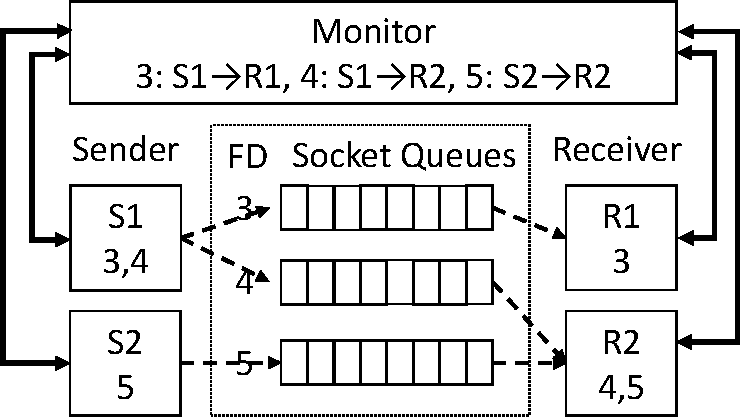
\includegraphics[width=0.6\textwidth]{images/queue_arch}
	\caption{Two sender threads and two receiver threads share a token-based socket. The dashed arrows represent the active sender and receiver for each socket. Each thread tracks its active sockets and communicates with the monitor through an exclusive queue.}
	\label{socksdirect:fig:queue-arch}
\end{figure}

%\RED{Need performance comparison in a figure.}

Detailed information for each type of operation is as follows: a) data transmission (\texttt{send} and \texttt{recv}), b) adding new senders and receivers (\texttt{fork} and thread creation), c) container hot migration, and d) connection closure.

\subsubsection{Send/Receive Operations}
\label{socksdirect:subsubsec:fork_rdwr}

\iffalse
\begin{figure}[htbp]
	\centering
	\subfloat[Traditional locking.]{
		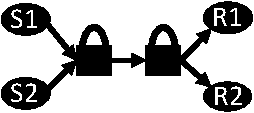
\includegraphics[width=0.3\textwidth]{images/one_conn3}
		\label{socksdirect:fig:fork-locking}
	}
	\hspace{0.02\textwidth}
	\subfloat[\sys{} one per sender.]{
		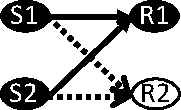
\includegraphics[width=0.22\textwidth]{images/one_conn1}
		\label{socksdirect:fig:fork-p2p}
	}
	\hspace{0.02\textwidth}
	\subfloat[S2 forks into S2' and S3]{
		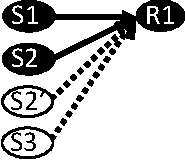
\includegraphics[width=0.2\textwidth]{images/one_conn2}
		\label{socksdirect:fig:fork-fork}
	}
	\caption{Inter-process queue structure of shared sockets. Dashed arrows represent queues that are not enabled.}
	\label{socksdirect:fig:inter-process-queue}
\end{figure}
\fi

When a thread does not have a send token but wants to send through a socket, the non-active thread needs to \emph{take over} the token. If a direct communication channel is created between the non-active thread and the active thread, it requires point-to-point queues, the number of which is the square of the number of threads, or a shared queue with locks. To avoid these two overheads, a monitor is used as a proxy during the \emph{takeover} process. Since takeover is an infrequent operation, the monitor generally does not become a bottleneck. This message passing design also has the following advantages: the sender process can be located on different hosts, which is very useful in container hot migration.

The takeover process is as follows: the non-active sender sends a \emph{takeover} command to the monitor through the shared memory queue. The monitor polls messages from various shared memory queues, adds the sender to the waiting list, and proxies the command to the current active sender. When the active sender receives the request, it sends the send token to the monitor. The monitor grants the token to the first non-active sender in the waiting list and updates the active sender. The non-active sender can send after receiving the token. This mechanism is deadlock-free because at least one sender or monitor holds the send token. It is also starvation-free because each sender can appear in the waiting list at most once and is served in FIFO order. The takeover process on the receiver side is similar.

The takeover process requires 0.6 microseconds, so if multiple processes send concurrently through the same socket, the total throughput may drop to 1.6 M operations per second. However, if we simply use locks, the throughput in the usual case will drop to 5 M operations per second, far lower than the 27 M operations per second throughput that can be achieved by token-based socket sharing.

%\begin{figure}[t]
%	\centering
%	
\includegraphics[width=0.3\textwidth]{images/fixme}
%	\caption{This figure shows a stable connection handled by multiple senders and receivers.}
%	\label{socksdirect:fig:fork-bipartitegraph}
%\end{figure}

\subsubsection{Fork, Exec and Thread Creation}
\label{socksdirect:subsubsec:fork_fork}

\textbf {Socket data sharing.}
The main challenge is to share socket metadata, buffers, and the underlying transport layer after \texttt {fork} and \texttt {exec}. After fork, the memory space becomes copy-on-write and is erased after exec, but the socket file descriptor still needs to be available. \sys{} uses shared memory to store socket metadata and buffers, so the data is still shared after fork. To attach shared memory after exec, \libipc {} connects to the monitor to get the shared memory key of its parent process. After fork, because the parent process cannot see the sockets created by the child process, the child process creates a new shared memory to store the metadata and buffers of the new socket.

Next, consider the underlying transport layer mechanism. The shared memory-based transport layer does not require special handling, as the shared memory created before fork / exec is still shared after fork / exec. However, there are problems with RDMA after fork / exec, because the DMA memory area is not in shared memory. They become copy-on-write after fork, and the network card still DMAs from the original physical page, so the child process cannot use the existing RDMA resources. After exec, the entire RDMA context will be cleared. The solution in this chapter is to let the child process reinitialize the RDMA resources (PD, MR, etc.) after fork / exec. When the child process uses a socket created before fork, it asks the monitor to re-establish the RDMA QP with the remote endpoint. Therefore, the peer process may see two or more QPs of a socket, but they link to the only copy of the socket metadata and buffer. In the next section (\S\ref{socksdirect:subsec:lockless-queue}), we will see that we only use the RDMA one-sided write primitive, so using any QP is equivalent. Figure \ref {socksdirect:fig:fork-memory} shows an example of fork.

\begin{figure}[htbp]
	\centering
	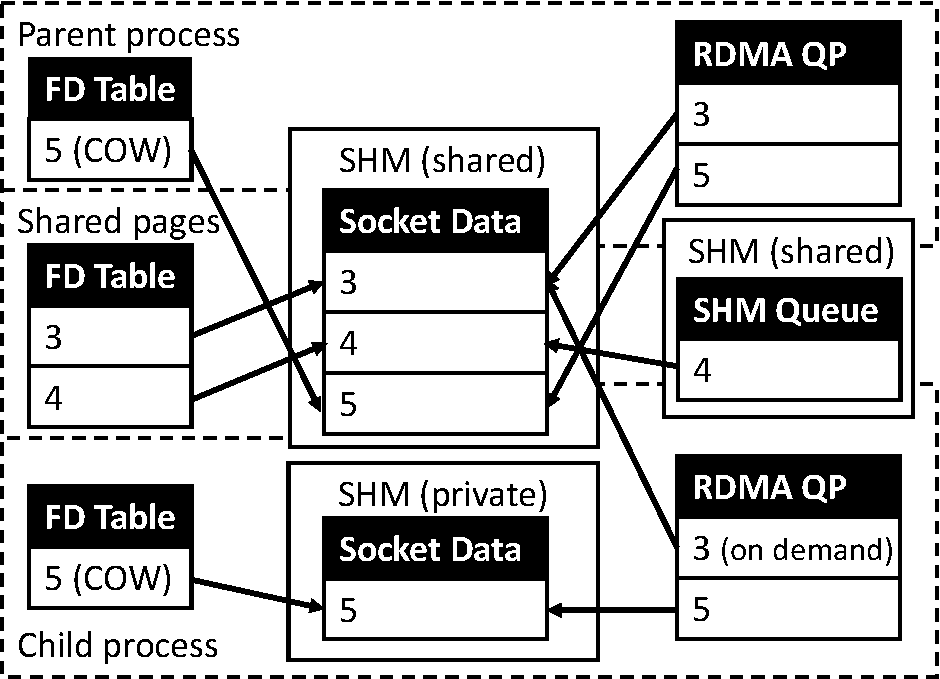
\includegraphics[width=0.6\textwidth]{images/fork_memory}
	\caption{Memory layout after fork. File descriptors 3 and 4 were created before fork and are therefore shared. After fork, the parent process and the child process each create a new file descriptor 5, which is copied on write in the file descriptor table. The socket metadata and buffers of file descriptors 3 and 4 are in shared memory and are therefore shared. The child process creates a new shared memory to store the socket metadata and buffers of file descriptor 5, which will be shared with the child process when it forks again. RDMA QP is in private memory, while the shared memory queue is shared.}
	\label{socksdirect:fig:fork-memory}
\end{figure}

\textbf {File descriptor space sharing.}
Unlike socket data, the file descriptor space becomes copy-on-write after fork: file descriptors created before fork are shared, but new file descriptors are exclusive to the creating process. Therefore, just keep the file descriptor remapping table in heap memory, taking advantage of the operating system's copy-on-write mechanism after fork. To restore the file descriptor remapping table after exec, it is copied to shared memory before exec and copied back to the new process during \libipc {} initialization.

\textbf{Security.}
Security is an issue because a malicious process may masquerade as a child process of a privileged parent process. To identify parent-child relationships in the monitor, when an application calls \texttt {fork}, \texttt {clone}, or \texttt {pthread\_create}, \libipc {} first generates a key for pairing and sends it to the monitor, then calls the original function in \emph {libc}. After fork, the child process creates a new shared memory queue for the monitor and sends the key (the child process inherits the parent memory space, thus knowing the key). Therefore, the monitor can pair the child process with the parent process.

\textbf {Monitor operations.}
During fork, exec, or thread creation, the monitor needs to add the new process to the sender and receiver lists of each existing socket to manage takeover operations.

%A more difficult challenge arises from the sharing of socket connections between parent and child processes.
%A significant challenge is how to manage the remaining data in the original send and receive queues.

%For each unidirectional queue, we examine the behavior of related processes in four scenarios:
%\begin{enumerate}
%	\item A sender process itself initiates a fork.
%	\item A receiver of a sender process initiates a fork.
%	\item A receiver process itself initiates a fork.
%	\item A sender of a receiver process initiates a fork.
%\end{enumerate}

%The general procedure of a fork is that, after the monitor is notified of the fork, it creates shared memory between the newly created process and all the processes that previously had connections with the parent process. The key challenge in the fork is how to handle the existing data in the connection to ensure the order requirements are met.

%\textbf{Receiver fork.}
%First, we consider a simple case where a receiver initiates a fork. Remember that only one receiver has exclusive access to a socket, as stated in Sec.~\ref{socksdirect:subsubsec:fork_rdwr}. The parent process inherits the receive permission. When a sender receives a fork notification from its peer, it copies all data from the original queues to the new queues of the parent process.

%\textbf{Sender fork.}
%When a sender initiates a fork, the situation becomes more complex. We need to ensure that all data sent before the \texttt{fork} is consumed before the data sent after the \texttt{fork}.

%Our solution is to allow receivers to drain the original queue first before switching to the new queues. After the \texttt{fork}, both the parent and child send data to their new queue. When the receiver is notified of the fork, it keeps track of the original queue and consumes all data in it before activating the new queues. Note that the parent or child may initiate another fork before the original queue is drained. With this in mind, the receiver maintains a forest data structure to track the dependency of queues. The root of each tree in the forest is the oldest queue to receive from. Each non-leaf node has two children indicating the new queue of parent and child processes. If a non-leaf root queue becomes empty, it will be removed, and the two children queues will be promoted to root nodes.

\subsubsection{Container Live Migration}
\label{socksdirect:subsubsec:container_live_migration}

\textbf{Migrating Remaining Data in Socket Queue.}
Since \libipc {} runs in the same process as the application, its memory state will be migrated to the new host along with the application.
The memory state includes the socket queue, so data in transit (sent but not received) will not be lost.
Sockets can only be shared within a container, and all processes in the container are migrated together, so the memory on the original host can be deallocated after migration.

\textbf{Migration of Monitor State.}
The monitor tracks information about listening sockets, active threads, and the waiting list for each connection as well as shared memory keys.
During migration, the old monitor dumps the state of the migrated container and sends them to the new monitor.

\textbf{Establishing New Communication Channels.}
After migration, all communication channels are obsolete, because shared memory is local on the host, and RDMA does not support live migration \cite{nsdi19freeflow,slim}.
First, the migrated container on the new host needs to establish a connection with the local monitor.
The local monitor instructs the following process.
A host-internal connection between two containers may become host-external, so \libipc {} creates an RDMA connection in this case.
A host-external connection between two containers may become host-internal, \libipc {} creates a shared memory connection.
Finally, \libipc {} re-establishes the remaining host-external RDMA and host-internal shared memory connections.

%\subsubsection{Connection Creation}
%\label{socksdirect:subsubsec:fork_new}
%

%A connection created by a thread can be accessed by all threads in the same process.
%To avoid creating redundant queues and connection states, \libipc does not share the file descriptor eagerly with other threads, because most threads in existing applications do not use connections created by other threads.
%When a thread do want to accesses a file descriptor that belongs to another thread, \libipc sends a message to the owner thread and requests sharing the file descriptor. %This procedure is exactly the same as sharing existing connections during thread creation (Sec.~\ref{socksdirect:subsubsec:fork_fork}). %The sharing procedure only happens once for every connection and thread. Sharing existing connections eagerly during thread creation is an optimization. First, children threads are more likely to use existing connections than siblings. Second, batch processing improves performance.

%\subsubsection{Connection Close}
%\label{socksdirect:subsubsec:fork_close}
%

%Close is the operation where all of the processes leave the connection. The synchronization is especially challenging since all the processes are run in parallel. One challenge lies in the fact that file descriptors are managed by decentralized processes and can possibly be reused. A case in point is when one process closes a connection while the others are performing compute-intensive tasks. It is possible that the file descriptor of the old process is reused and a new connection is set up with the same file descriptor. The other process may notice the closure of the old connection and also call close on its own side, which leads to the new connection set up by the previous process being closed due to the match of the same file descriptor. 

%To satisfy the synchronization requirements, the close function call is all completed by message passing. The caller of close needs to wait for ACK from all the other peers before releasing resources, i.e., the status of the connection.

%\textbf{Broadcast.}
%When a process calls \texttt{close}, all its peers cannot send to or receive from the file descriptor. In this sense, 
%A socket is closed if all shared processes close it. Therefore, we need to multicast a notification to the peers and collect responses from them. A challenge arises when \texttt{close} is interleaved with \texttt{fork}. Since \texttt{fork} and \texttt{close} do not commute~\cite{clements2015scalable}, we need a rule to determine their partial order. We make the choice that the ordering is determined by the initiator of \texttt{close}. If a process calls \texttt{close} before receiving fork notification, it will piggyback close notification with fork completion to both parent and child processes.

%\textbf{Handshake before releasing resource.}
%Another challenge is caused by file descriptor reuse after close. As stated in Sec.~\ref{socksdirect:subsec:socket-api}, a file descriptor is deleted after receiving shutdown message of both directions. With multiple processes sharing a connection, after one process calls \texttt{close}, others can still use the connection. Consequently, a process deletes a file descriptor only after receiving shutdown messages of both directions from all peers of the file descriptor.

%Another challenge lies in the termination of a connection, as termination is a broadcast operation while send/receive is directed to a specific process. Furthermore, fork and termination are immutable operations, while the scalability requirements of the system impose the constraint that all operations run asynchronously. Consequently, a rule to determine the partial order is necessary.

%In \libipc, we opt for the order of fork and termination to be determined at the initiation point of the fork operation and the termination point (after receiving all the ACKs). By making this choice, when a process waiting for fork termination ACK encounters a fork message, it can send a separate termination request to the newly created process, ensuring all processes are terminated.
